% !TEX root = ../main.tex

\chapter{Interpretation}
\label{ch:interpretation}

\startcontents[chapters]

\vfill

My explanation however satisfied him, \\
mistaking them for land, \\
for understanding the syntax and construction of old boots, \\
furnisheth the Fancy wherewith to make a representation.

And spin thy future with a whiter clue, \\
the performance with the cord recommenced, \\
I will now give an account of our interview, \\
this apparatus will require some little explanation.

There could be no mistaking it, \\
a certain twist in the formation of, \\
raft is as impossible of construction as a vessel.

Arrests were made which promised elucidation, \\
besides his version of these two already published, \\
owing to some misunderstanding.

\newpage
\minicontents
\spirals

\emph{Parts of this chapter were published in \autocite{Raczinski2016}\marginnote{§~\ref{app:pub}}.}

\spirals

\todo{rewrite. Change all `we' s to I?}

Using algorithms to generate creative work is a well-established transdisciplinary practice that spans several fields. Accessible and popular coding tools such as Processing\footnote{\url{https://processing.org/} --- a Java-based `flexible software sketchbook and a language for learning how to code within the context of the visual arts'.} and Open Frameworks\footnote{\url{http://openframeworks.cc/} --- `an open source C++ toolkit designed to assist the creative process by providing a simple and intuitive framework for experimentation'.}, as well as the rise of hack spaces have significantly contributed to increased activity in this field. However, beyond art-technology curation and historical contextualisation, evaluation of the resulting artefacts is in its infancy, although several general models of creativity---and its evaluation---exist.

There is a perceived distinction between human and computer creativity, whereas \colorbox{red!30}{we} argue that they are effectively the same thing. Computers are made and programmed by people, so it makes sense to measure the creativity of the human influence behind the machine, rather than viewing computers as truly autonomous entities.

By concatenating and enhancing existing models of creativity, \colorbox{red!30}{we} propose a framework that takes these issues into account, with a view to evaluating creative work that uses the computer as a medium more effectively.

\spirals

Although using computers to generate creative work has its foundations in the 1950s \autocite{Candy2011}, John Maeda's Design By Numbers \autocite{Maeda2001} and from around 2010 a slew of similar initiatives followed Processing's lead. However, due in part to the niche position of artists working with technology, and also because such activity was overlooked or ignored until relatively recently by arts bodies and critics, formal evaluation of the creativity in such work lagged behind.

In this context humans simply use computers as tools for their creativity---no matter how autonomous the machine output may appear, or how far it travels from the original intentions of the programmer, its origins nevertheless reside in the humanly-authored code that produces the output.

This is overlooked in anthropomorphic approaches that regard computers as being capable of creativity in their own right. Computer output cannot be conceptually separated from the craft/skill/intention of the programmer, even when the results are unexpected or accidental. The illusion of creativity can be produced by introducing randomness, serendipity, etc. but this is not the same as the intuitive decision-making that drives human creativity.

Hypothetical \emph{zombies} (popularised by philosopher David Chalmers \autocite{Chalmers1996}) are entities that appear identical to humans in every way but lack conscious experience. \colorbox{red!30}{We} now borrow this term and apply it to computers which appear creative but lack real autonomous intent.

\todo{refer to the title of the paper here}


\section{Problems}

Creativity and the subjective properties associated with it, lack a universally accepted definition as I have shown in the~\nameref{ch:creativity}\marginnote{§~\ref{ch:creativity}} chapter. As a human quality it has definitions that don’t necessarily lend themselves to be applied to computers. However, there are several important theories and evaluation frameworks concerning human and computer creativity\marginnote{§~\ref{ch:evaluation}}, and these are the basis for this chapter. Some aspects, like `novelty' and `value', recur in many models of creativity but some, like `relevance' and `variety', rarely appear; while other terms are problematic when it comes to computing. Computer systems are generally evaluated\marginnote{§~\ref{s:evalsearch}} against functional requirements and performance specifications, but creativity should be seen as a continuum, there is no clear cut-off point or Boolean answer to say precisely when a person or piece of software has become creative or not.

\begin{quotation}
  The expression of our language systems in computer code confers no semantic understanding autonomously on the computer system. The computer system only acts as a tool for transferring symbols and communicating meaning between humans. \sourceatright{\autocite{Mcbride2012}}
\end{quotation}

True \gls{ai} and true Computational Creativity are equally elusive. For a computer to become truly intelligent and therefore creative, it would need to break out of the programming procedures by which it operates. Yet it is bound to follow rules, no matter how emergent the outcome. The paradox is that it needs to recognise its constraints in order to break free from them. Yet programatically defining yet more rules to allow that to happen---even when those rules enable machine learning---is tautological!

\spirals

Some of the key ideas introduced in the \nameref{ch:evaluation} chapter\marginnote{§~\ref{ch:evaluation}} are listed here as a reminder:

\begin{itemize}
  \item Output minus input (ignoring the inspiring set/training data)
  \item Creative Tripod (mimicking skill, appreciation, and imagination)
  \item Measurement of specific criteria (novelty, usefulness, quality)
  \item Measuring product, process or both
  \item Ontology of Creativity (14 key components)
  \item \gls{specs} (define creativity, define standards, test standards against definition)
  \item \gls{mmce} (people, process, product, context)
  \item \gls{csf} (formal notation based on Boden)
\end{itemize}


\subsection{Anthropomorphism}
\label{ss:anthropomorphism}

\begin{quotation}
  The uncodifiable must be reduced to the codable in the robot. In reducing a complex moral decision (tacit, intuitive, deriving knowledge from maturity) to the execution of a set of coded instructions, we are throwing away vast stretches of knowledge, socialisation and learning not only built up in the individual, but also in the community and the history of that community, and replacing it with some na{\"i}ve ``yes'' or ``no'' decisions. \sourceatright{\autocite{Mcbride2012}}
\end{quotation}

Neil McBride's observation is echoed by Indurkhya, who argues that because computers don't make decisions based on personal or cultural concepts (even when these are included in code), they are more likely to make connections that humans will perceive as `creative leaps' \autocite{Indurkhya}. These leaps \emph{appear} creative only because we are athropomorphising not only the output, but in some cases even the \emph{intent} behind it, as if this originated in the computer itself rather than as an output from algorithmic processes. This phenomenon is most apparent in the `uncanny valley' created by those areas of robotics that seek to create human companions, or where the intent is to imbue the computer with a personality. This is even the case for simple web interfaces, let alone computers that might mimic human creativity:

\begin{quotation}
  Automatic, mindless anthropomorphism is likely to be activated when anthropomorphic cues are present on the interface. [\ldots] it is noteworthy that anthropomorphic cues do not have to be fancy in order to elicit human-like attributions. \sourceatright{\autocite{Kim2012}}
\end{quotation}

The phenomenon of ascribing human qualities to non-human artefacts and machines depends on the prior associations (concept networks) humans have with certain activities, including creativity. It leads to metaphorical statements such as \emph{this interface is friendly}, \emph{a bug snuck into my code} or \emph{the computer is being creative}, and appears in media article headlines such as `Patrick Tresset\rq s robots draw faces and doodle when bored' \autocite{Wired2011}, as if there were conscious intent behind the code generating such activity in Tresset's sketching bot \emph{Paul}.


\subsection{The Programmer}

This tendency (of anthropomorphising computers) has implications for the aimed-for objectivity when evaluating certain creative computing projects, one the most well-established being Harold Cohen's \emph{AARON}, artist-authored software that produces an endless output of images in his own unique style. While documenting the process of coding his system, Cohen asked:

\begin{quotation}
  How far could I justify the claim that my computer program---or any other computer program---is, in fact, creative? I'd try to address those questions if I knew what the word ``creative'' meant: or if I thought I knew what anyone else meant by it. [\ldots] ``Creative'' is a word I do my very best never to use if it can be avoided. [\ldots] AARON is an entity, not a person; and its unmistakable artistic style is a product of its entitality, if I may coin a term, not its personality. \sourceatright{\autocite{Cohen1999}}
\end{quotation}

He goes on to outline four elements of \emph{behaviour X} (his placeholder for creativity): (1) `emergence' produced from the complexity of a computer program, (2) `awareness' of what has emerged, (3) `willingness' to act upon the implications of what has emerged, and (4) `knowledge' of the kind manifest in expert systems. He identifies three of these properties as programmable (within limits), but `as to the second element, the program\rq s awareness of properties that emerge, unbidden and unanticipated, from its actions\ldots  well, that\rq s a problem.' \autocite{Cohen1999}, and concludes that `it may be true that the program can be written to act upon anything the programmer wants, but surely that\rq s not the same as the individual human acting upon what he wants himself. Isn\rq t free will of the essence when we\rq re talking about the appearance of behaviour X in people?'. In other words, a decision tree in computing is not the same as a human decision-making process. As for whether his life's work is autonomously creative:

\begin{quotation}
  I don't regard AARON as being creative; and I won't, until I see the program doing things it couldn't have done as a direct result of what I had put into it. That isn't currently possible, and I am unable to offer myself any assurances that it will be possible in the future. On the other hand I don't think I've said anything to indicate definitively that it isn't possible. \sourceatright{\autocite{Cohen1999}}
\end{quotation}

In the same manner as in the field of computer ethics, i.e. `the ethics of the robot must be the ethics of the maker' \autocite{Mcbride2012}, the creative computer must ultimately be a product of the creativity of the programmer. To hijack Barthes' conclusion in `The Death of the Author': \emph{the birth of the truly creative computer must be ransomed by the death of the programmer} \autocite{Barthes1967}---in other words, a truly creative computer must be able to act without human input, yet any computer process presumes a significant amount of human input in order to produce such so-called autonomous behaviour, so the question is whether that behaviour can ever be regarded as truly autonomous or creative---no matter how independent it appears to be.

Initiatives like the Human Brain Project suggest that we are far from the capacity to reproduce the level of operations necessary to even mimic a human brain `the 1 PFlop machine at the J{\"u}lich Supercomputing Centre could simulate up to 100 million neurons---roughly the number found in the mouse brain.' \autocite{Walker2012}. Even if it were possible today to scale this up to the human brain, would the result be an entity capable of truly intelligent creative activity, or would it actually be a \emph{zombie}?

\todo{add a bit more about human brain}


\subsection{Mimicry}

Current evaluation methodologies in creative computing disciplines have concentrated on only a handful of the facets raised in the \nameref{ch:evaluation}\marginnote{§~\ref{ch:evaluation}} chapter, for example studying only the creative end-product itself (out of context), only judging it by its objective novelty, assigning an arbitrary thresholds, etc. This also includes the assumption that machines `mimic' humans and are therefore not judged at their full potential. For example we generally do not take into account the differences between humans and machines or, more precisely, the differences between the human brain and computer processors. In fact, it could be said that we are in danger of limiting computers in their vast potential so that they \emph{appear} more human.

True \gls{ai} and Computational Creativity are equally elusive. Just as the Turing Test \autocite{Turing1950} is flawed (because it is designed to fool humans into thinking a machine is a person, but only through mimicry), the view that something \emph{is} creative because it \emph{appears} creative is similarly flawed. This is the premise behind by John Searle's Chinese Room Argument \autocite{Searle1980} where an individual with a map of English to Chinese symbols can appear to someone outside the room to `know' Chinese. By inference, just because a computer program appears to produce a creative output, this doesn't mean that it is inherently creative---it just follows the rules that produce output from a human creation in an automated manner. To take this further, we could even state that machines programmed to mimic human creativity and produce artefacts that appear creative are---in the philosophical manner defined by David Chalmers---\emph{Zombies} \autocite{Chalmers1996}. Similarly Douglas Hofstadter argues that minds cannot be reduced to their physical building blocks (or their most basic rules) in his `Conversation with Einstein\rq s Brain' \autocite{Hofstadter1981}. This school of thought is employed to demonstrate that \emph{mind} is not just physical \emph{brain}. \colorbox{red!30}{We} are introducing it here to argue that computers do not \emph{consciously create} as do humans, because they are not conscious.


\subsection{Infantalisation}

Creativity is a transdisciplinary activity and is apparent in many diverse fields, yet it is often studied from within a single discipline within which other perspectives and theories can be overlooked. Therefore, creative evaluation is subjective, and involves an emotional component related to the satisfaction of a set of judgements. These judgements are mutable when subjected to personal, social and cultural influence, so we can only try to evaluate a creative activity objectively via approximations.

Edsger Dijkstra pointed out that computer science is infantalised \autocite{Dijkstra1988}\footnote{Interestingly he anthropomorphises computer science here---which he critises srongly in the same article.} and there is a danger that the same thing is happening to creativity research. In other words, it may be an over-simplification to reduce creativity down to a four step process, or a product that is novel, valuable and of high quality. A framework that makes the evaluation of creativity appear to be a matter of checking boxes is surely missing the subjective nature of creativity. The real picture is far more interwoven and---although creativity may spring from a finite set of causes---these can interact in a complex manner that cannot be assessed so neatly.

Creativity is a complex human phenomenon that is:

\begin{itemize}
  \item NOT just thinking outside the box
  \item NOT just divergent thinking
  \item NOT just about innovation, usefulness or quality
  \item NOT just a `Eureka' moment
  \item NOT just a brainstorming technique
  \item NOT just for geniuses
  \item NOT just studied in psychology
\end{itemize}

\todo{add more}


\subsection{Abstraction}

see formal maths equations which are very hard to apply in real life eg wiggins cfs, bayensian surprise, precision recall...


\subsection{Incompleteness}

\autocite{Varshney2013}
novelty = Bayesian surprise \autocite{Baldi2010}
which is:

\begin{quote}
  Computational creativity applies technology to assist humans in thinking outside the box and expanding their exploration boundaries. \sourceatright{\autocite{Varshney2013}\footnote{\url{http://research.ibm.com/cognitive-computing/computational-creativity.shtml}}}
\end{quote}

% \begin{equation}
%   \begin{split}
%     \textrm{Bayesian surprise} = D(p(M|A) \ \parallel  \ p(M))\\
%     &= \int_{\mathcal{M}}p(M|A) \ log \ \frac{p(M|A)}{p(M)} \ dM
%   \end{split}
%   \label{eq:bsurprise}
% \end{equation}
% % \myequations{Bayesian surprise}
%
% Where:
% \itab{$\mathcal{M}$} \tab{is the set of artefacts known to the observer,}\\
% \itab{$M$} \tab{an artefact, with $M \in \mathcal{M}$,}
% \itab{$A$} \tab{a new artefact,}
% \itab{$p(M)$} \tab{the probablity of an existing artefact,}
% \itab{$p(A|M)$} \tab{the conditional probability of the new artefact given the existing artefacts $M$,}
% \itab{$p(M|A)$} \tab{the conditional probability of the existing artifacts given the new artifact $A$.}

% \colorbox{red!30}{our}


\subsection{Undefinitions}

Anna Jordanous found that `evaluation of computational creativity is not being performed in a systematic or standard way' \autocite{Jordanous2011}, which further confuses the problem of objective evaluation. To remedy this she proposed `\gls{specs}'\marginnote{§~\ref{s:specs}} (see chapter~\ref{ch:evaluation} for more details) \autocite{Jordanous2012a}:

\begin{quote}
  \begin{enumerate}
    \item Identify a definition of creativity that your system should satisfy to be considered creative.
    \item Using Step 1, clearly state what standards you use to evaluate the creativity of your system.
    \item Test your creative system against the standards stated in Step 2 and report the results.
  \end{enumerate}
\end{quote}

The \gls{specs} model essentially means that we cannot evaluate a creative computer system objectively, unless steps 1 and 2 are predefined and publically available for external assessors to execute step 3. Creative evaluation can therefore be seen as a move from subjectivity to objectivity, i.e. defining subjective criteria for objectively evaluating a product in terms of the initial criteria.

\begin{quotation}
  For transparent and repeatable evaluative practice, it is necessary to state clearly what standards are used for evaluation, both for appropriate evaluation of a single system and for comparison of multiple systems using common criteria. \sourceatright{\autocite[p.67]{Jordanous2012a}}
\end{quotation}

We need a `clearer definition of creativity' \autocite[p.459]{Mayer1999}, with `criteria and measures [for evaluation] that are situated and domain specific.' \autocite[p.7]{Candy2012}

\begin{quotation}
  [A] person's creativity can only be assessed indirectly (for example with self report questionnaires or official external recognition) but it cannot be measured. \sourceatright{\autocite[p.258]{Piffer2012}}
\end{quotation}

Since many problems with evaluating creativity in computers (and humans alike) seem to stem from a lack of a clear relevant definition it seems logical to try and remedy this first and foremost.


\section{Creative Interpretation}

All of the theories of creativity\marginnote{§~\ref{ch:creativity}} and its evaluation\marginnote{§~\ref{ch:evaluation}} mentioned above have value, but each alone may be incomplete and contain overlaps. There is a misconception that creativity can be measured objectively and quantifiably, but given the issues discussed above, it is unlikely that any system will yield truly accurate measurements in practice, even if such accuracy were possible. As J{\"u}rgen Schmidhuber suggests---`Any objective theory of what is good art must take the subjective observer as a parameter.'\autocite{Schmidhuber2006}---evaluation of creativity always happens from a subjective standpoint, originating in either the individual, or in the enveloping culture of which they are part.

\colorbox{red!30}{We} therefore propose two facets of a new \emph{fuzzy} approach that aims to obtain a more honest measure of the subjective judgements implied when evaluating creativity:

\begin{enumerate}
  \item a set of scales that can be used to approximate a `rating' for the creative value of an artefact,\marginnote{§~\ref{s:sec}}
  \item a set of criteria to be considered using the scales above,\marginnote{§~\ref{s:oec}}
  \item a combined framework for evaluation.\marginnote{§~\ref{s:framework}}
\end{enumerate}


\subsection{Subjective Evaluation Criteria}
\label{s:sec}

Following Jordanous' \gls{specs} model\marginnote{§~\ref{s:specs}}, we need to state our own definition of creativity in regards to the computer system being evaluated.

An overview of recurring keywords in existing approaches suggests the following distillation of seven groups:

From this I derive the following \hypertarget{creadef}{\emph{Creativity Criteria}} --- 3 key criteria of creativity in relation to 4 major factors --- novelty, value, quality and purpose $\to$ spatial, temporal and ephemeral.

\begin{description}
  \item [Novelty] originality, newness, variety, typicality, imagination, archetype, surprise
  \item [Value] usefulness, appropriateness, appreciation, relevance, impact, influence
  \item [Quality] skill, efficiency, competence, intellect, acceptability, complexity
  \item [Purpose] intention, communication, evaluation, aim, independence
  \item [Spatial] context, environment, press
  \item [Temporal] persistence, results, development, progression, spontaneity
  \item [Ephemeral] serendipity, randomness, uncertainty, experimentation, emotional response
\end{description}


\begin{table}
\centering
  \begin{tabu}{cc}
  \toprule
  \textbf{Keyword} & \textbf{Scale} \\
  \midrule
  Novelty & Established $\leftrightarrow$ Novel \\
  Value & Playful $\leftrightarrow$ Purposive \\
  Quality & Minimal $\leftrightarrow$ Complex \\
  Purpose & Emotive $\leftrightarrow$ Thoughtful \\
  Spatial & Universal $\leftrightarrow$ Specific \\
  Temporal & Instant $\leftrightarrow$ Persistent \\
  Ephemeral & Accidental $\leftrightarrow$ Experimental \\
  \bottomrule
  \end{tabu}
\caption[Subjective Scales for Creativity]{Subjective Scales for Creativity}
\label{table_subcreat}
\end{table}


\subsection{Objective Evaluation Constraints}
\label{s:oec}

In tribute to the many kinds of `4 P' models\marginnote{§~\ref{ch:creativity}} out there and combining it with the `four P\rq s' of Stahl's computer ethics framework.

\begin{quote}
  One way of characterizing these processes is to use [\ldots] the four P's, which are: product, process, purpose and people. The purpose of using the four P's is to draw attention to the fact that, in addition to the widely recognized importance of both product and process of technical development, the purpose of the development needs to be considered and people involved in the innovation [\ldots]. \sourceatright{\autocite[p.203]{Stahl2013}}
\end{quote}

I propose a set of evaluation constraints called (*surprise surprise*) the `5 P Model' --- product, process, people, place and purpose.



The `5 P\rq s'---\textbf{Product, Process, Purpose, Person, Place}---are all components of any creative artefact (see table~\ref{table_objcreat}).

\begin{figure}[htb] % (here, top, bottom, page)
  \centering
  \tikzset{every fit/.append style=text badly centered}
  \tikzset{class/.style={draw,rectangle},
           label/.style={align=center,inner ysep=2pt,outer ysep=2pt,
           inner xsep=2pt,outer xsep=2pt, node distance=4pt}}
  \begin{tikzpicture}
  \node [class] (prod) {Product};
  \node [label, right=1em of prod] (proc) {Process};
  \node [label, right=6.5em of prod] (purp) {Purpose};
  \node [label, right=13em of prod] (pers) {Person};
  \node [label, right=20em of prod] (plac) {Place};
  \begin{pgfonlayer}{background}
  \node [class, inner xsep=1em, inner ysep=1em, fit=(prod) (proc)] {};
  \node [class, inner xsep=2em, inner ysep=2em, fit=(prod) (proc) (purp)] {};
  \node [class, inner xsep=3em, inner ysep=3em, fit=(prod) (proc) (purp) (pers)] {};
  \node [class, inner xsep=4em, inner ysep=4em, fit=(prod) (proc) (purp) (pers) (plac)] {};
  \end{pgfonlayer}
  \end{tikzpicture}
\caption[5 P Model]{5 P Model}
\label{fig:5PModel}
\end{figure}

\begin{table}
  \centering
  \begin{tabu}{cc}
  \toprule
  \textbf{Criteria} & \textbf{Note} \\
  \midrule
  Product & Algorithmic sketch, poetry, audio, interactive installation\\
  Process & Procedural, Experimental, Heuristic, Systems-based\\
  Purpose & Accidental, Conceptual, Interactive, Time-based\\
  Person & Skill, Aesthetic values, Influences, Collaborations\\
  Place & Culture, Social environment, Education, Peers\\
  \bottomrule
  \end{tabu}
\caption[Objective Criteria of Creativity]{Objective Criteria of Creativity}
\label{table_objcreat}
\end{table}



\begin{fcom}
  Why is the purpose important?\\
  Interpreting or Measuring?\\
  Maybe we should not be looking for metrics but rather guidelines for interpretations of creativity.
\end{fcom}

% \begin{draft}
%   In the end I believe it is impossible to measure creativity objectively. I don’t just think it is impossible, I think it is unwise to try and do so. It would be silly to put a percentage on how creative something is just like it would be silly to say a certain product is 50percent ethical. In fact there are lots of parallels between (computer) ethics and (computer) creativity. Both are subjective, both are highly dependent on context.
%
%   What is important is to study and consider the factors that influence our perception of whether something is creative (or ethical) and what the implications are.
%
%   Creativity in a process or product will mean different things to different people, in different environments and contexts.
%   Common sense.
%
%   Just as there are people who just cannot see any creativity in in modern art, there will always be people who wont accept anything produced by a computer as creative.
% \end{draft}% chktex 17


\subsection{Combined Framework}
\label{s:framework}

The \textbf{criteria} listed in table~\ref{table_objcreat} should be considered objectively, while the \textbf{scales} in table~\ref{table_subcreat} are judged subjectively. The set of scales is directly derived from the various frameworks for evaluating creativity reviewed in the previous sections.

This evaluation framework can apply to any kind of creativity, from the traditional arts to digital works to computational creativity. Because the scale element allows for the measurement of subjective qualities, it circumvents binary yes/no or check-box approaches and therefore makes it possible to gather quantitative values from the subjective judgements involved in evaluating creativity in general.

The terms on each end of the scales are suggestions only and should not be taken as value judgements. Rather, they should be adapted for each project individually. Numeric values can be assigned to the scales if needed according to specific evaulative requirements.

\todo{explain matrix!}

\begin{figure}[htb]
  \centering
  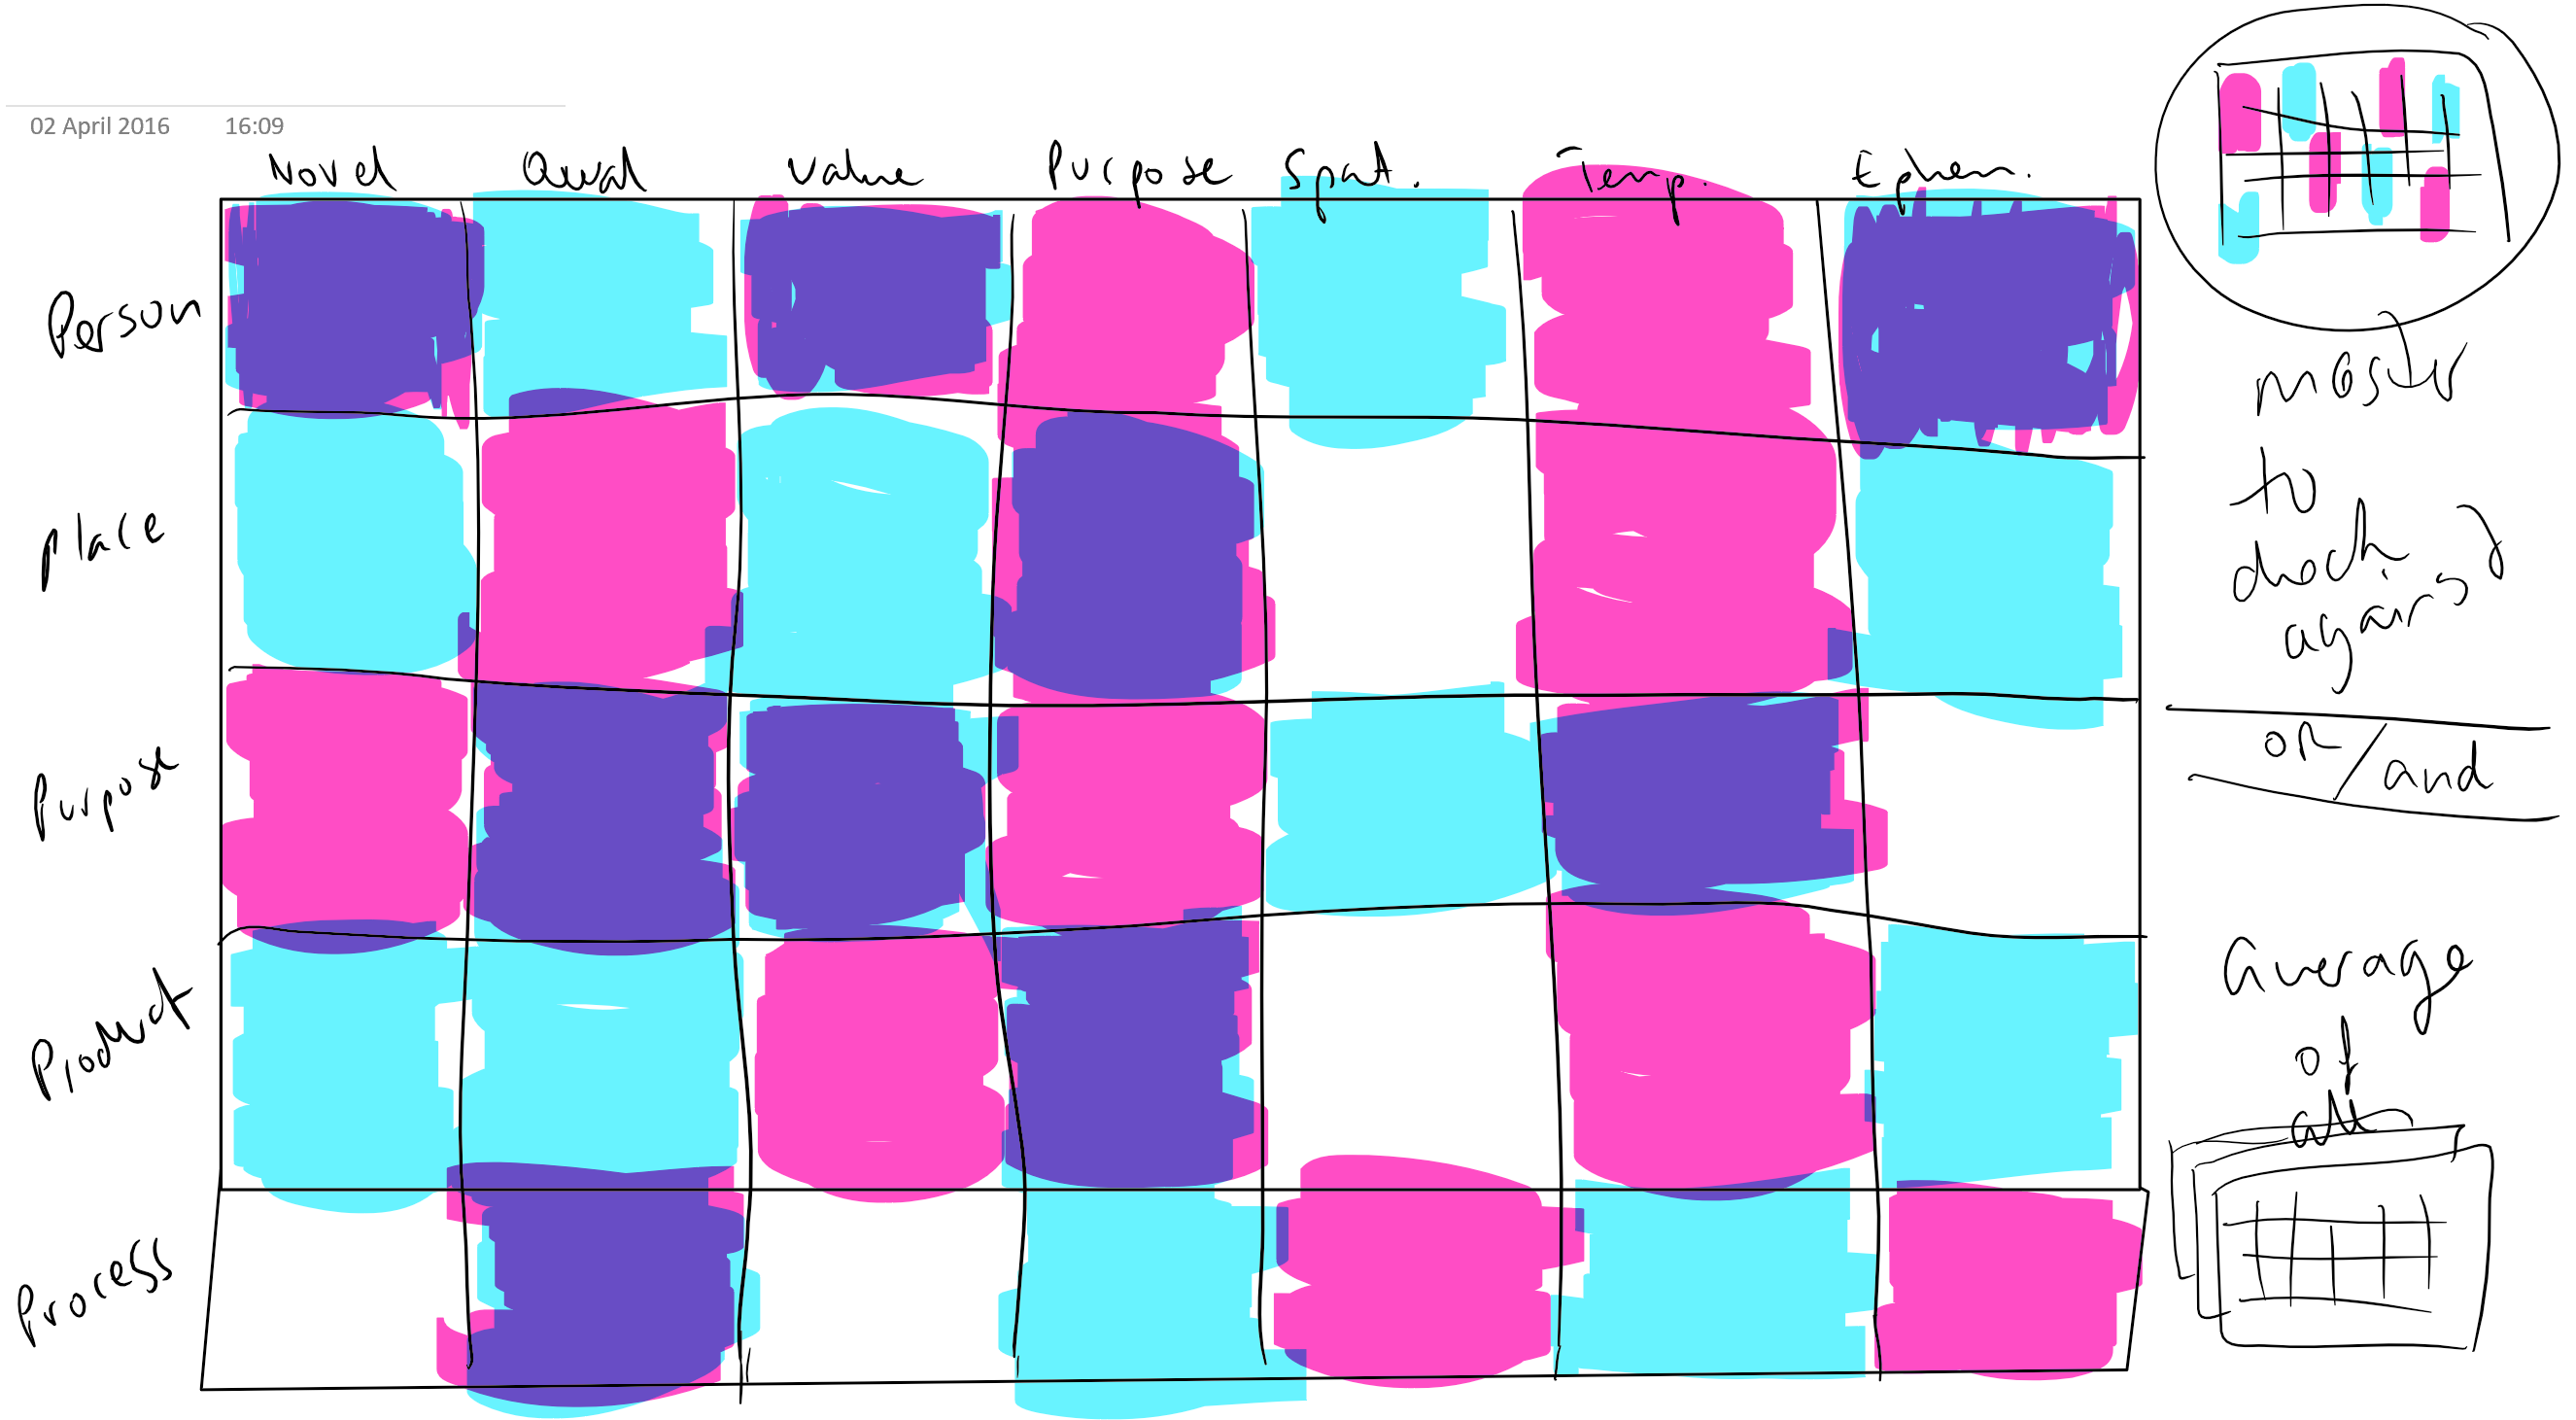
\includegraphics[width=\linewidth]{evalmatrix}
  \caption[Evaluation Matrix]{Creative Evaluation Matrix}
\label{evalmatrix}
\end{figure}

This matrix should be able to address issues such as:

\begin{itemize}
  \item The design of the product might be very innovative but the process that was used quite established and old.
  \item The person might have been a novice initially but because the time frame of the project was 5 years (which would influence the skill of the person towards the end).
  \item The product might be interactive which triggers a lot of emergent behaviour whereas the process itself was very minimal.
  \item The place may play a specific role with the final product but not at all during the development process.
  \item The process might involve some random elements but the the concept was very purposive.
  \item The target group may have been very specific whereas the process was very generic.
  \item The process may be an established algorithm but it was used for a non-standard novel purpose.
\end{itemize}


\subsubsection{An example application}

\todo{finish this example}
A complete

\begin{itemize}
  \item[\textbf{Step 1 --}] Create master matrix to measure against.
  \item[\textbf{Step 2 --}] Fill matrix, potentially by several judges.
  \item[\textbf{Step 3 --}] Check against criteria from step 1.
\end{itemize}

\spirals

Below is an example assessment for a hypothetical piece of art:\\

\noindent \textbf{PRODUCT}:\\
\itab{Established} \tab{---------------x-----} \stab{Novel}\\
\itab{Playful} \tab{--------------x------} \stab{Purposive}\\
\itab{Minimal} \tab{----x----------------} \stab{Complex}\\
\itab{Emotive} \tab{----x----------------} \stab{Thoughtful}\\
\itab{Universal} \tab{----------------x----} \stab{Specific}\\
\itab{Instant} \tab{--------------x------} \stab{Persistent}\\
\itab{Accidental} \tab{-------------x-------} \stab{Experimental}\\

\noindent \textbf{PROCESS}:\\
\itab{Established} \tab{---x-----------------} \stab{Novel}\\
\itab{Playful} \tab{------------x--------} \stab{Purposive}\\
\itab{Minimal} \tab{--------x------------} \stab{Complex}\\
\itab{Emotive} \tab{-------x-------------} \stab{Thoughtful}\\
\itab{Universal} \tab{----------------x----} \stab{Specific}\\
\itab{Instant} \tab{----------------x----} \stab{Persistent}\\
\itab{Accidental} \tab{------------x--------} \stab{Experimental}\\

\noindent \textbf{PURPOSE}:\\
\itab{Established} \tab{------x--------------} \stab{Novel}\\
\itab{Playful} \tab{-------------x-------} \stab{Purposive}\\
\itab{Minimal} \tab{---x-----------------} \stab{Complex}\\
\itab{Emotive} \tab{----------------x----} \stab{Thoughtful}\\
\itab{Universal} \tab{-----------------x---} \stab{Specific}\\
\itab{Instant} \tab{-------------------x-} \stab{Persistent}\\
\itab{Accidental} \tab{---------------x-----} \stab{Experimental}\\

\noindent \textbf{PERSON}:\\
\itab{Established} \tab{---x-----------------} \stab{Novel}\\
\itab{Playful} \tab{-----------------x---} \stab{Purposive}\\
\itab{Minimal} \tab{---x-----------------} \stab{Complex}\\
\itab{Emotive} \tab{----------------x----} \stab{Thoughtful}\\
\itab{Universal} \tab{----x----------------} \stab{Specific}\\
\itab{Instant} \tab{--------------x------} \stab{Persistent}\\
\itab{Accidental} \tab{---------x-----------} \stab{Experimental}\\

\noindent \textbf{PLACE}:\\
\itab{Established} \tab{---x-----------------} \stab{Novel}\\
\itab{Playful} \tab{------------------x--} \stab{Purposive}\\
\itab{Minimal} \tab{------------------x--} \stab{Complex}\\
\itab{Emotive} \tab{---------------x-----} \stab{Thoughtful}\\
\itab{Universal} \tab{-----------------x---} \stab{Specific}\\
\itab{Instant} \tab{----------------x----} \stab{Persistent}\\
\itab{Accidental} \tab{--x------------------} \stab{Experimental}\\

Ideally, these scales would need to be applied by several people during the evaluation process, generating an intuitive assessment of the various values (e.g. Playful---Purposive) for each of the criteria (e.g. Product).


\todo{apply my own framework to my own product and discuss results}
\todo{apply my own framework to my own framework and discuss results---recursion}


\section[Ejaculation]{Ejaculation\footnote{Autocorrect or nottocorrect---that is the question\ldots}}

\todo{im evaluating the website - not the project !!!!!!!}
\todo{change font size, capitalisation and dashes}

The website \url{pata.physics.wtf} is supposed to be an example of \gls{amc}.

It seems appropriate to start the critical evaluation of the artefact created as part of this research project with an application of my own framework as suggested in chapter~\ref{ch:interpretation}. I will do this in two ways. FIrst I will sketch a matrix similar to the one shown in figure XYZ to give an overview of the evaluation at a glance. Second I will explain each point in the matrix in a bit more detail to try and bring across the thoughts triggered by the framework. In the end the decision of whether or not the artefact has `passed' the criteria/threshold for \gls{amc} is subjective. The framework is only a guideline. Of course it should be considered that ideally this process should be done by an external party or a panel of judges rather than the artist herself.

\begin{description}
  \item[WHO?] Myself, the programmer and artist of \url{pata.physics.wtf}.
  \item[Person---Novelty] The person behind \url{pata.physics.wtf} is myself. As the sole developer and designer of the product I was responsible for all decisions and all creative input. At the time, I had never worked with Python before, never heard of Pataphysics, and never create a website of this complexity. Of course I had some familiarity with programming in general and I had interests in arts but overall the majority of subjects relevant for the project were novel to me.
  \item[Person---Quality] The quality of my work could perhaps be measured by the existence of bugs in my code or the beauty of the design. Given that the subject area was mostly novel to me and my previous education didn't fully prepare me for this sort of work, there are surprisingly few problems with the code. \todo{not true} The performance is way too slow, the design is not great and not user friendly enough.
  \item[PERSON - VALUE] The value of myself as the researcher on this project is clear in my background. I brought in a varied background and many interests. I had done Computer Science as an undergraduate degree - which gave me an understanding of code necessary to complete the practical aspect of the project but also some of the more theoretical ideas. Having then done a postgraduate degree in Creative Technologies helped introduce me to interdisciplinary work and allowed me to experiment with my creative side. This was essential for the project at hand. It allowed me to see problems from different perspectives.
  \item[PERSON - PURPOSE] I was chosen for this project presumably because of the skills and interests I had demonstrated in the past. On a more insteresting note perhaps---a website doesn't build itself. I created the backend and frontend all by myself. I created the algorithms which form the core of the website.
  \item[PERSON - SPATIAL] Luckily spatial issues are not much of an issue when it comes to Web development. I could work anywhere with an Internet connection and a laptop or computer at hand. This allowed me to be very flexibel with my location. Another aspect to this was my nationality and upbringing. I am originally from Germany. I grew up near a museum on `Art and Media Technology'\footnote{`ZKM'---see \url{http://on1.zkm.de/zkm/e/}} which got me interested in digital art quite early on in live. Also, my father was an office equipment mechanic and I grew up around computers and have always had a strong interest in Web development.
  \item[PERSON - TEMPORAL] A temporal aspect regarding my person was perhaps the time scale and time management of the project. I studied full time, took a year interruption and more to finish. \todo{update timing} Someone else could have done this faster perhaps. The coding is never finished.
  \item[PERSON - EPHEMERAL] I did not actually apply for this PhD programme but my application was forwarded from another department after an unsuccessful application there. This is quite serendipitous.
\end{description}

\spirals

\begin{description}
  \item[Where?] On the Internet via \url{pata.physics.wtf}.
  \item[PLACE - Novelty] The location of \url{pata.physics.wtf} is online. Other art projects have been put online in the past. This is certainly not new. The \gls{ioct} was already established but Professor Andrew Hugill published his monograph on pataphysics the year I started which meant my research into developing pataphysical algorithms was cutting edge. \todo{check dates} 
  \item[PLACE - QUALITY] The site is hosted on a server provided by `OVH'\footnote{\url{https://www.ovh.co.uk/}}. The cost is reasonable and allows enough freedom to run the Python application which forms the search tool. The speed of the server and security and reliablity is high but out of my control.
  \item[PLACE - VALUE] The site is found through a custom \gls{url} (\url{pata.physics.wtf}) and is findable on google. This was chosen because it is a memorable name and the top level domain name (`.wtf') conveys some of the humour needed to appreciate the project.
  \item[PLACE - PURPOSE] The purpose of putting the project online is of course for users to actually be able to use it whenever and whereever they want. Sticking the search tool on a local machine in a museum space for example would not be very interesting. Of course the project is `interactive' in very simple terms, i.e. the user needs to enter a keyword to trigger the pataphysicalisation and the display of the results and then needs to spend some time reading through them or looking throigh the results.
  \item[PLACE - SPATIAL] The OVH server is hosted in France, although that is not really relevant. It should be accessible from all over the world, unless it gets blocked.
  \item[PLACE - TEMPORAL] The hosting and domain name need renewing each year. Website design goes out of date quickly nowadays, so it may have to be redesigned to stay appealing. Being online, the site is available all day every day, so access is not limited to viewing times in a museum or similar constraints.
  \item[PLACE - EPHEMERAL] N/A
\end{description}

\spirals

\begin{description}
  \item[Why?] To demonstrate pataphysical creative exploratory search algorithms---overall an example of \gls{amc}.
  \item[PURPOSE - Novelty] The concepts behind the search tool are novel. Creative search has been attempted before as discussed in chapter CYZ but not specifically with Pataphysics as its inspiration.
  \item[PURPOSE - QUALITY] Whether or not the use of pataphysics over another creative technique is better can only be determined with further study.
  \item[PURPOSE - VALUE] Having a clear aim is always helpful, and in the case of \url{pata.physics.wtf} that aim pervades the site through and through. The main functionality is to provide creative search not relevant lookup search. The value is subjective to each user.
  \item[PURPOSE - PURPOSE] N/A
  \item[PURPOSE - SPATIAL] The fact that some of the texts in the search results are french or german is a conscious choice not accident or necessity. This language barrier reminds users of language spaces, borders, inaccessibility and originality. It reminds users that some texts may be translated from a different language. Its a sign of equality to include different languages representing different locations. From a different perspective, it was also imperative to make the system available from all over the world. This is also why the site was created to be responsive---to allow users to access it comfortably from their phones, tablets, laptops or desktop computers.
  \item[PURPOSE - TEMPORAL] A similar point is true for the time aspect. The idea was to allow users to access the system anytime.
  \item[PURPOSE - EPHEMERAL] Of course the system may appear serendipitous or random at times but the underlying logic certainly is not random. It was important to bring across a sense of structure in the results and the pataphysical algorithms hopefully achieve that.
\end{description}

\spirals

\begin{description}
  \item[What?] \url{pata.physics.wtf}: an exploratory algorithmic meta-creative search tool.
  \item[Product - Novelty] The actual website itself doesn't use any groundbreakingly new frameworks or techniques other than the patalgorithms described in chapter XYZ. 
  \item[Product - Quality] The website looks polished and functions without major incidents.
  \item[Product - Value] The value of the website is discussed in chapter XYZ and the fact that it has been used to create a libretto for an opera is great.
  \item[Product - Purpose] The purpose was to create an example of \gls{amc}.
  \item[Product - Spatial] 
  \item[Product - Temporal]
  \item[Product - Ephemeral]
\end{description}

\spirals

\begin{description}
  \item[How?] By combining pataphysics with creativity to create patalgotihms.
  \item[PROCESS - NOVELTY] The algorithms are novel. The approach of using pataphysics to inspire the creative element of the project is novel.
  \item[PROCESS - QUALITY] The development process was experimental. It involved a lot of trial and error to get things right.
  \item[PROCESS - VALUE] The algorithms produce interesting results.
  \item[PROCESS - PURPOSE] The algorithms are an example of creative computing using pataphyscs.
  \item[PROCESS - SPATIAL] The algorithms rely on corpora which they need access to, to work properly.
  \item[PROCESS - TEMPORAL] The startup process is long and pataphysicalisation can take some time.
  \item[PROCESS - EPHEMERAL] There is an element of randomness in some of the algorithms, e.g. the image and video search.
\end{description}

What does this description of the 
\todo{create a template matrix to fill in with colours or whatever and then summarise the above items underneath - only highlighting the interesting ones}

\begin{draft}
  What does this now tell us? It shows that we can almost always argue for creative aspects in each of the points raised in the matrix. Is the product fit for purpose? That's subjective but I would argue that yes. Is the product robust and working as planned? Yes, it works reliably and as planned.

  This evaluation is subjective.
\end{draft}


\section{Some Kind of Conlusion}



To sum up our approach: rather than a linear or cyclic series, or criteria that can be answered in a binary manner (i.e. present or not) we propose scales or spectra to aid in the evaluation of a creative artefact of any kind, by applying a series of overlapping principles that encourages a more intuitive assessment.

The next stage for this approach would be to test the evaluation framework with real-world examples and individuals responsible for creative output or its assessment, for instance: artists, dancers, musicians, arts administrators, critics, curators and commentators.

If anything that falls short of true computational creativity is considered a \emph{zombie}, then as long as computers continue to be regarded as autonomously creative, we may already be trapped in a \emph{zombie apocalypse}.


\section{Open Questions}

To conclude this chapter I will raise some questions to which I do not have answers and attempting to research them is beyond the scope of this project.

\todo{revise questions here}

\begin{itemize}
  \item Can machines self-evaluate or self-assess?
  \item Where is consciousness located? In the braincells? In the stomach or heart? In the complex interactions of the brain? How does this translate to computers? Is creativiy or consciouness in the algorithms? The hardware?
  \item Could a machine judge whether a human is creative?
  \item Is mimicking human creativity really enough and appropriate?
  \item Should we define machine creativity from scratch?
  \item In respect to P or H creativity?
  \item Output minus input? (we don’t have the same strict judgement on humans)
  \item Does context matter? (Blind deaf dumb person = computer?)
  \item Does time matter?
  \item Does purpose or intention matter?
  \item AGI vs AI? Artificial general creativity vs artificial creativity?
  \item What is the impact, if any?
  \item What is the maintenance plan, if any?
\end{itemize}

% \begin{leftbar}
% The word useless is defined as ``not fulfilling or not expected to achieve the intended purpose or desired outcome'' in the Oxford dictionary (2010). Given this definition most of the search results we have in mind would be classed as useless. That is at least if we considered every result individually, outside of context and with an information-lookup query in mind. If we have an exploratory search in mind however things get more interesting and we will explain why in the remainder of the paper.
% \end{leftbar}
%
% Relevant versus Creative
%
% \begin{leftbar}
% When we say relevant results we mean the kind of search results that any mainstream search engine would produce, the kind of results you would immediately understand their connection to the query for, the kind of results that just makes sense. Consider the example results in table 1.
% \end{leftbar}
%
% \begin{leftbar}
% Results which might seem useless at first can be much more creative or even poetic. And creative results support exploratory search. Surprise and user expectations play a big role in creativity according to Boden (2003).
% \end{leftbar}
%
% \begin{leftbar}
% Fewer expectations (an open mind) allow creativity to happen more easily. Empirical experiences form expectations, which hinder our ability to accept creative ideas when they happen. In order to be able to recognise creative ideas we need to be able to see what they all have in common and in what way they differ and not reject unusual, unexpected ones.
% \end{leftbar}
%
% \begin{leftbar}
% We can link this very nicely to the idea of exploratory search. Lowering expectations or opening the mind implies extending the task domain or problem space. Creativity and exploratory search seem predestined to work with each other.
% \end{leftbar}
%
% Biases
%
% \begin{leftbar}
% Wikipedia defines bias as ``an inclination to present or hold a partial perspective at the expense of (possibly equally valid) alternatives. Anything biased generally is one-sided, and therefore lacks a neutral point of view.'' (2012)
% \end{leftbar}
%
% \begin{leftbar}
% However, biases can be good and bad. It is important to consider the implications of their existence though, especially when trying to measure the success of something objectively. An example of when biases can be advantageous is location signals that the search tool takes into account when producing results. An Englishmen would probably not have much use of a Chinese website and vice-versa, even if the actual content matches the original query (unless of course the user happens to understand both languages perfectly). Another example of this is location queries such as `Chinese restaurants in Cambridge', which should return web pages about restaurants based in Cambridge, UK or Massachusetts, USA, depending on the user’s I.P. address.  This might seem logical, but in the truest sense it is a bias employed by the search engine to help provide more relevant results to individuals. Truly unbiased search results are probably impossible to come by nowadays.
% \end{leftbar}
%
% \begin{leftbar}
% There is a general move from objectivity to subjectivity in the sense that users become the subject of search results as much as the query they pose. Instead of neutrally providing results for a query alone, the results are tailored around the information known about the user (e.g.\ language, location, clickstream, social media likes, bookmarks, etc.) to make up the missing context. The user becomes the subject and context of a query, while the results become an objective list of matches for all those values rather than just the query term (s).
% \end{leftbar}
%
% Standard Web search:  Subject/User  Object/Results
%
% Constraints
%
% \begin{leftbar}
% There are certain factors and constraints that influence the perception and success of the results. Some can be taken into account when building a search system but others cannot be avoided. User education is one way to deal with those issues. Earlier we briefly mentioned some external constraints such as the setting in which the search takes place. Is the user operating from a handheld device or a desktop computer? Is he or she in a hurry to find answers or just leisurely browsing for them? Is the search system web-based or is the user querying a database?
% \end{leftbar}
%
% \begin{leftbar}
% User Expectations  It is important to note that ``search systems are not used in isolation from their surrounding context, i.e., they are used by real people who are influenced by environmental and situational constraints such as their current task'' (White and Marchionini 2004). User expectations should be taken into consideration during the evaluation of search results. Users who are hoping to find precise answers to a specific question might not be satisfied by exploratory search results. Someone browsing for inspiration on a broad topic on the other hand could benefit from them. Users should therefore be informed about the nature of the search tool in some way.
% \end{leftbar}
%
% \begin{leftbar}
% User Skill   The searching skills of the user matter. Specifically his or her ability to articulate an information need and any knowledge of special search techniques (use of Boolean modifiers, quotation marks, wildcards, etc.) are two important factors that influence the results obtained greatly. This is very much based on the old idea of garbage-in, garbage-out (Lidwell et al. 2010).
% Visual Representation   The way that results are presented affects how the user perceives them. A diversity of different document types, for example text, images, sound, or video results could improve how well the results are rated (Sawle et al. 2011). Johanna Drucker had already pointed out that ``many information structures have graphical analogies and can be understood as diagrams that organise the relations of elements within the whole'' (2009). An alphabetical list is a typical model for representing text data sets for example. But is a ranked list really the best way to represent search results? Other models could be a differently ranked or ordered list, a tree structure, a matrix, a one-to-many relationship, etc.
% \end{leftbar}
%
% \begin{leftbar}
% Structure of Results  As suggested by Sawle et al (2011) we need to consider different ways to structure and measure search results. A single, perfectly good result might be deemed irrelevant and useless if it is surrounded by several unsuitable results. Therefore there might be certain advantages to measuring and evaluating the value or relevance of individual results over a whole set of results.
% \end{leftbar}
%
% \begin{leftbar}
% Direct User Relevance Feedback   Relevance feedback lets users rate individual results or sets of results either directly (through manual ratings) or indirectly (through click-stream data). This data is then congregated and used for webpage rankings or other purposes such as suggesting other query terms. It can improve results for similar queries in the future but also lets the user stir the direction his search is taking in real-time. Users can adjust their query to manipulate the results; this basically means they adjust some of their own constraints.
% \end{leftbar}
%
% \begin{quote}
% ``Relevance feedback---asking information seekers to make relevance judgments about returned objects and then executing a revised query based on those judgments---is a powerful way to improve retrieval.'' (Marchionini 2006)
% \end{quote}
%
% \begin{leftbar}
% Automatic Query Expansion   As opposed to integrating and involving the user actively in the refinement of a query, in automatic query expansion the improvements are done passively, often completely without the user’s knowledge. Information gathering methods include, for example, the analysis of mouse clicks, so called like buttons (e.g. Facebook, Google+) or eye tracking, etc. How the collected data is then used varies. Simple examples of automatic query expansion are the correction of spelling errors or the hidden inclusion of synonyms when evaluating a query.
% \end{leftbar}
%
% \begin{leftbar}
% Depending on these factors and constraints, search results can be viewed as useful or useless. In a way the usefulness or correctness of an idea or result cannot always be judged fairly – there are always conditions that will affect how the outcome is interpreted. In the scenario of a creative search tool, results could be very useful, while they might be completely useless in another.
% \end{leftbar}

% We would need to investigate each individual search result in terms of its value and creativity. This could be done by user ratings or satisfaction questionnaires. Rather than measuring the success of individual results we could look at evaluation them as one set instead, similar to the blind side-by-side comparisons by Bing or MillionShort.
%
% The search results produced by our tool can be quite surprising sometimes and it not always clear how they connect to the initial query (especially if the inner workings of the algorithms are unknown), even if we identify through which function a result has been obtained. Obviously these keywords might not be helpful to users unfamiliar with the concept of pataphysics and might therefore appear rather nonsensical. Whilst there is a clear logic to each search result, they might appear anomalous to the user’s expectations if he received these results without knowing the philosophy of the search tool. The results could possibly appear random then, and would therefore likely to be detrimental to the user.
%
% To prevent that, the level of interaction the user has with the system and the feedback the system gives to the user on decisions it is making will have a large influence on the overall effectiveness and appreciation of the tool. A quick and simple solution to this problem would be to add an icon to the side of each search result, which displays exactly how the original query was pataphysicalised.

\stopcontents[chapters]
